    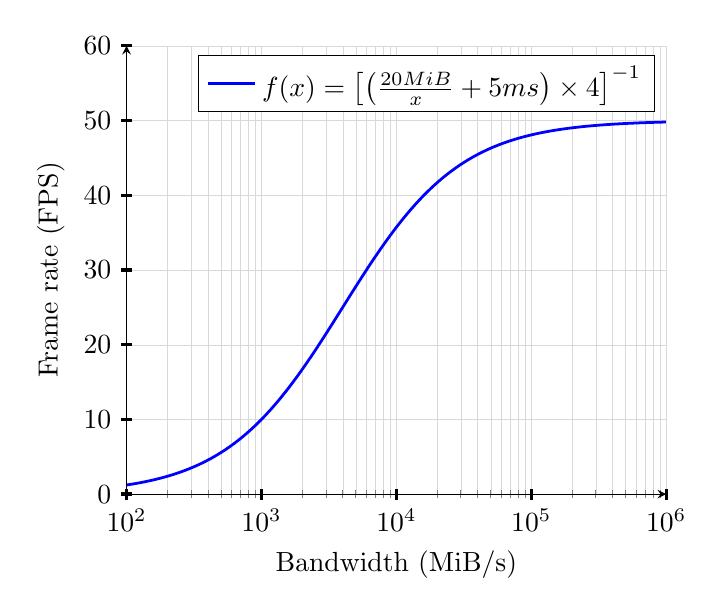
\begin{tikzpicture}
    \begin{semilogxaxis}[
        axis lines = left,
        xlabel = {Bandwidth (MiB/s)},
        ylabel = {Frame rate (FPS)},
        ymin = 0, ymax = 60,
        xmin = 100, xmax = 1000000,
        ytick distance=10,
        grid=both,
        grid style={line width=.1pt, draw=gray!30},
        every major tick/.append style={very thick, major tick length=4pt, black},
    ]
    
    \addplot [
        domain=1:1000000, 
        samples=1000, 
        color=blue,
        line width=1pt
    ]
    {1/((20/x + 0.005)*4)};
    
    \addlegendentry{$f(x) = \left[ \left( \frac{\SI{20}{MiB}}{x} + \SI{5}{ms} \right) \times 4 \right]^{-1}$}
    \end{semilogxaxis}
    \end{tikzpicture}
